\documentclass{article}

\usepackage{fancyhdr}
\usepackage{extramarks}
\usepackage{amsmath}
\usepackage{amsthm}
\usepackage{amsfonts}
\usepackage{tikz}
\usepackage[plain]{algorithm}
\usepackage{algpseudocode}
\usepackage{graphicx}
\usepackage{mcode}
\usetikzlibrary{automata,positioning}

%
% Basic Document Settings
%

\topmargin=-0.45in
\evensidemargin=0in
\oddsidemargin=0in
\textwidth=6.5in
\textheight=9.0in
\headsep=0.25in

\linespread{1.1}

\pagestyle{fancy}
\lhead{\hmwkAuthorName}
\chead{\hmwkClass\ (\hmwkClassInstructor\ \hmwkClassTime): \hmwkTitle}
\rhead{\firstxmark}
\lfoot{\lastxmark}
\cfoot{\thepage}

\renewcommand\headrulewidth{0.4pt}
\renewcommand\footrulewidth{0.4pt}

\setlength\parindent{0pt}

%
% Create Problem Sections
%

\newcommand{\enterProblemHeader}[1]{
    \nobreak\extramarks{}{Problem \arabic{#1} continued on next page\ldots}\nobreak{}
    \nobreak\extramarks{Problem \arabic{#1} (continued)}{Problem \arabic{#1} continued on next page\ldots}\nobreak{}
}

\newcommand{\exitProblemHeader}[1]{
    \nobreak\extramarks{Problem \arabic{#1} (continued)}{Problem \arabic{#1} continued on next page\ldots}\nobreak{}
    \stepcounter{#1}
    \nobreak\extramarks{Problem \arabic{#1}}{}\nobreak{}
}

\setcounter{secnumdepth}{0}
\newcounter{partCounter}
\newcounter{homeworkProblemCounter}
\setcounter{homeworkProblemCounter}{1}
\nobreak\extramarks{Problem \arabic{homeworkProblemCounter}}{}\nobreak{}

%
% Homework Problem Environment
%
% This environment takes an optional argument. When given, it will adjust the
% problem counter. This is useful for when the problems given for your
% assignment aren't sequential. See the last 3 problems of this template for an
% example.
%
\newenvironment{homeworkProblem}[1][-1]{
    \ifnum#1>0
        \setcounter{homeworkProblemCounter}{#1}
    \fi
    \section{Problem \arabic{homeworkProblemCounter}}
    \setcounter{partCounter}{1}
    \enterProblemHeader{homeworkProblemCounter}
}{
    \exitProblemHeader{homeworkProblemCounter}
}

%
% Homework Details
%   - Title
%   - Due date
%   - Class
%   - Section/Time
%   - Instructor
%   - Author
%

\newcommand{\hmwkTitle}{Homework\ \#6}
\newcommand{\hmwkDueDate}{December 13, 2016}
\newcommand{\hmwkClass}{STAT 5444}
\newcommand{\hmwkClassTime}{}
\newcommand{\hmwkClassInstructor}{Professor Scott Leman}
\newcommand{\hmwkAuthorName}{Kevin Malhotra}

%
% Title Page
%

\title{
    \vspace{2in}
    \textmd{\textbf{\hmwkClass:\ \hmwkTitle}}\\
    \normalsize\vspace{0.1in}\small{Due\ on\ \hmwkDueDate\ }\\
    \vspace{0.1in}\large{\textit{\hmwkClassInstructor\ \hmwkClassTime}}
    \vspace{3in}
}

\author{\textbf{\hmwkAuthorName}}
\date{}

\renewcommand{\part}[1]{\textbf{\large Part \Alph{partCounter}}\stepcounter{partCounter}\\}

%
% Various Helper Commands
%

% Useful for algorithms
\newcommand{\alg}[1]{\textsc{\bfseries \footnotesize #1}}

% For derivatives
\newcommand{\deriv}[1]{\frac{\mathrm{d}}{\mathrm{d}x} (#1)}

% For partial derivatives
\newcommand{\pderiv}[2]{\frac{\partial}{\partial #1} (#2)}

% Integral dx
\newcommand{\dx}{\mathrm{d}x}

% Alias for the Solution section header
\newcommand{\solution}{\textbf{\large Solution}}

% Probability commands: Expectation, Variance, Covariance, Bias
\newcommand{\E}{\mathrm{E}}
\newcommand{\Var}{\mathrm{Var}}
\newcommand{\Cov}{\mathrm{Cov}}
\newcommand{\Bias}{\mathrm{Bias}}

\begin{document}

\maketitle

\pagebreak

\begin{homeworkProblem}
\lstinputlisting{Problem1.m}
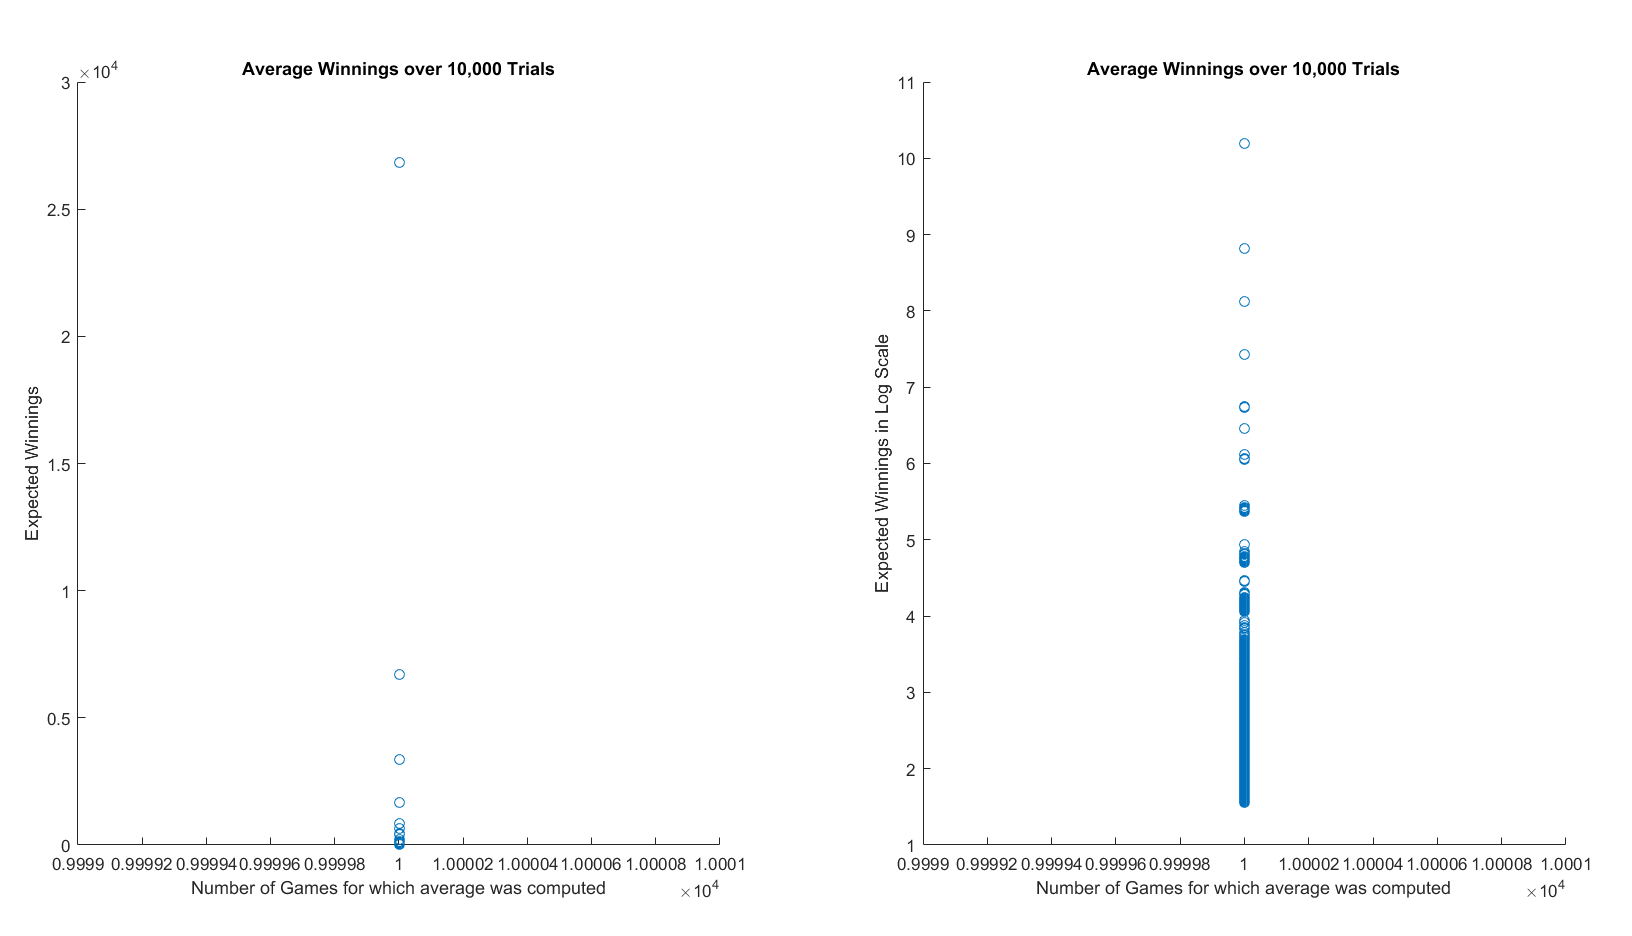
\includegraphics[scale=0.3]{avgGamesOverExpectedWinnings} \\
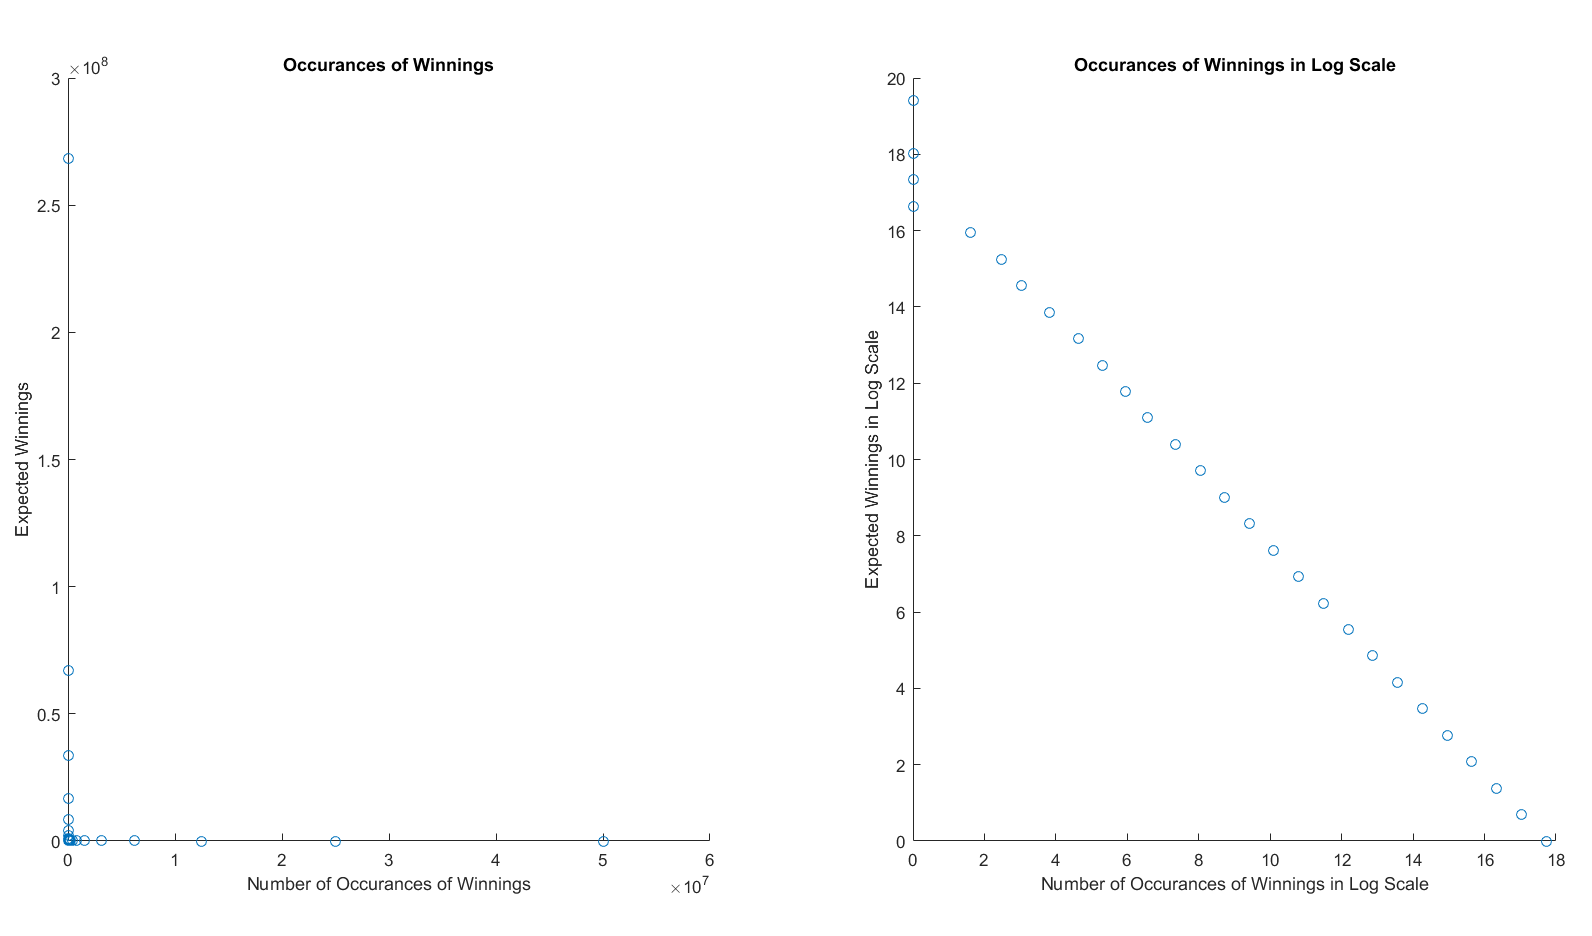
\includegraphics[scale=0.3]{occuranceWinnings} \\
I would be willing to spend to pay 1 dollar to play this game because there are not enough outcomes for higher winnings for me to win more than once. \\
\begin{align*}
E[U] &= \sum_{k=1}^\infty \frac{log(2^{k-1})}{2^k} \\
E[U] &= \sum_{k=1}^\infty \frac{(k-1)log(2)}{2^k} \\
E[U] &= log(2) \sum_{k=1}^\infty \frac{(k-1)}{2^k} \\
E[U] &= log(2) \sum_{k=1}^\infty \frac{(k-1)}{2^k} =1 * log(2) \\
\end{align*}
The summation converges to 1 by the ratio test. The log utility function was log(2) therefore the utility is 2 dollars. 
\end{homeworkProblem}
\begin{homeworkProblem}
A Bayes estimator uses the posterior and the loss over the entire parameter space and it is minimized such that the Bayes estimator is better on average. A proper prior has different weights over the parameter space and will sum to one. A improper prior (flat priors) will not always sum to one. Thus, there has to be some part in the parameter space which will yield that the Bayes estimator is better due to the different weights on a proper prior. This will yield a lower loss which can be translated to a lower risk on average, therefore at some point the bayes estimator must be admissible somewhere.
\end{homeworkProblem}
\begin{homeworkProblem}
Assume \(e^\pi\) is not minmax such that there exist some estimator \( R(e^\pi, \theta) = C > max_\theta R(e, \theta) \). \(e^\pi\) is dominating the other risk which means it is inadmissible. Because Bayes estimators are admissible by contradiction \(e^\pi\) is minmax.
\end{homeworkProblem}
\end{document}
